\section*{Problem 2: (2,3)-Bäume und (2,4)-Bäume} 


\textbf{a)} Fügen Sie die Schlüssel A, L, G, O, D, T, S, X, Y, Z in dieser Reihenfolge in einen anfangs leeren (2, 3)-Baum ein. Löschen Sie sodann die Schlüssel Z, A, L. Zeichnen Sie den Baum nach jedem Einfüge- und Löschvorgang, und zeigen Sie die Modifikation, welche durchgeführt werden. \\


Ein (2,3)-Baum hat folgende Grenzen:
\begin{itemize}
\item min children: 2, max children: 3
\item min entries: 1, max entries: 2
\item A,B,C,D,E,F,G,H,I,J,K,L,M,N,O,P,Q,R,S,T,U,V,W,X,Y,Z
\end{itemize}

\begin{multicols}{2}

\begin{enumerate}

\item insert(A):

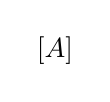
\begin{tikzpicture}[scale=0.5,
  level 1/.style={sibling distance=40mm},
  level 2/.style={sibling distance=20mm},
  level 3/.style={sibling distance=20mm},
  level 4/.style={sibling distance=20mm}]
\node{$[A]$};
\end{tikzpicture}

\item insert(L):

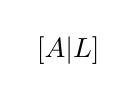
\begin{tikzpicture}[scale=0.5,
  level 1/.style={sibling distance=40mm},
  level 2/.style={sibling distance=20mm},
  level 3/.style={sibling distance=20mm},
  level 4/.style={sibling distance=20mm}]
\node{$[A|L]$};
\end{tikzpicture}

\item insert(G):

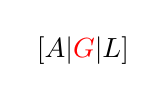
\begin{tikzpicture}[scale=0.5]
\node{$[A|\textcolor{red}{G}|L]$};
\end{tikzpicture}\\
$\Rightarrow$ Die Wurzel hat zu viele Einträge $\rightarrow$ Splitten

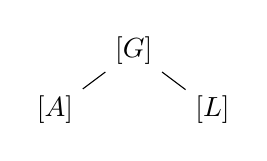
\begin{tikzpicture}[scale=0.5,
  level 1/.style={sibling distance=20mm},
  level 2/.style={sibling distance=20mm},
  level 3/.style={sibling distance=20mm},
  level 4/.style={sibling distance=20mm}]
\node{$[G]$}
	child{node{$[A]$}}
	child[missing]
	child{node{$[L]$}};
\end{tikzpicture}\\

\item insert(O):

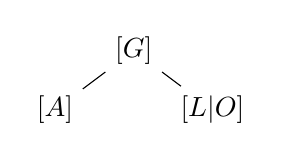
\begin{tikzpicture}[scale=0.5,
  level 1/.style={sibling distance=20mm},
  level 2/.style={sibling distance=20mm},
  level 3/.style={sibling distance=20mm},
  level 4/.style={sibling distance=20mm}]
\node{$[G]$}
	child{node{$[A]$}}
	child[missing]
	child{node{$[L|O]$}};
\end{tikzpicture}\\

\item insert(D):

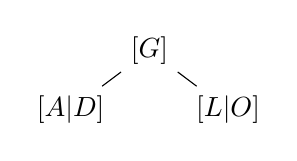
\begin{tikzpicture}[scale=0.5,
  level 1/.style={sibling distance=20mm},
  level 2/.style={sibling distance=20mm},
  level 3/.style={sibling distance=20mm},
  level 4/.style={sibling distance=20mm}]
\node{$[G]$}
	child{node{$[A|D]$}}
	child[missing]
	child{node{$[L|O]$}};
\end{tikzpicture}\\


\item insert(T):

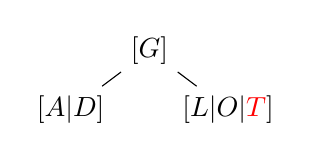
\begin{tikzpicture}[scale=0.5,
  level 1/.style={sibling distance=20mm},
  level 2/.style={sibling distance=20mm},
  level 3/.style={sibling distance=20mm},
  level 4/.style={sibling distance=20mm}]
\node{$[G]$}
	child{node{$[A|D]$}}
	child[missing]
	child{node{$[L|O|\textcolor{red}{T}]$}};
\end{tikzpicture}\\

$\Rightarrow$ Das rechte Blatt $[L|O|T]$ hat zu viele Einträge $\rightarrow$ Rebalance

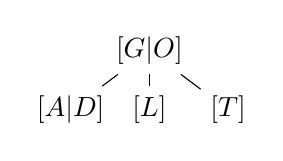
\begin{tikzpicture}[scale=0.5,
  level 1/.style={sibling distance=20mm},
  level 2/.style={sibling distance=20mm},
  level 3/.style={sibling distance=20mm},
  level 4/.style={sibling distance=20mm}]
\node{$[G|O]$}
	child{node{$[A|D]$}}
	child{node{$[L]$}}
	child{node{$[T]$}};
\end{tikzpicture}\\


\item insert(S):

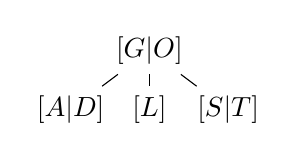
\begin{tikzpicture}[scale=0.5,
  level 1/.style={sibling distance=20mm},
  level 2/.style={sibling distance=20mm},
  level 3/.style={sibling distance=20mm},
  level 4/.style={sibling distance=20mm}]
\node{$[G|O]$}
	child{node{$[A|D]$}}
	child{node{$[L]$}}
	child{node{$[S|T]$}};
\end{tikzpicture}\\

\item insert(X):

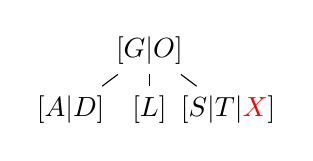
\begin{tikzpicture}[scale=0.5,
  level 1/.style={sibling distance=20mm},
  level 2/.style={sibling distance=20mm},
  level 3/.style={sibling distance=20mm},
  level 4/.style={sibling distance=20mm}]
\node{$[G|O]$}
	child{node{$[A|D]$}}
	child{node{$[L]$}}
	child{node{$[S|T|\textcolor{red}{X}]$}};
\end{tikzpicture}\\

$\Rightarrow$ Das rechte Blatt $[S|T|\textcolor{red}{X}]$ hat zu viele Einträge $\rightarrow$ Rebalance

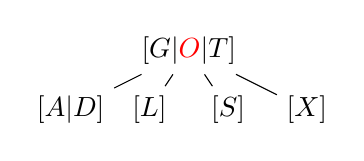
\begin{tikzpicture}[scale=0.5,
  level 1/.style={sibling distance=20mm},
  level 2/.style={sibling distance=20mm},
  level 3/.style={sibling distance=20mm},
  level 4/.style={sibling distance=20mm}]
\node{$[G|\textcolor{red}{O}|T]$}
	child{node{$[A|D]$}}
	child{node{$[L]$}}
	child{node{$[S]$}}
	child{node{$[X]$}};
\end{tikzpicture}\\

$\Rightarrow$ Die Wurzel hat zu viele Einträge \& zu viele Kinder $\rightarrow$ Rebalance

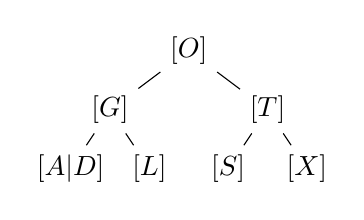
\begin{tikzpicture}[scale=0.5,
  level 1/.style={sibling distance=40mm},
  level 2/.style={sibling distance=20mm},
  level 3/.style={sibling distance=20mm},
  level 4/.style={sibling distance=20mm}]
\node{$[O]$}
	child{node{$[G]$}
		child{node{$[A|D]$}}
		child{node{$[L]$}}}
	child{node{$[T]$}
	child{node{$[S]$}}
	child{node{$[X]$}}};
\end{tikzpicture}\\

\item insert(Y):

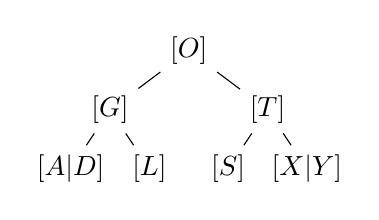
\begin{tikzpicture}[scale=0.5,
  level 1/.style={sibling distance=40mm},
  level 2/.style={sibling distance=20mm},
  level 3/.style={sibling distance=20mm},
  level 4/.style={sibling distance=20mm}]
\node{$[O]$}
	child{node{$[G]$}
		child{node{$[A|D]$}}
		child{node{$[L]$}}}
	child{node{$[T]$}
	child{node{$[S]$}}
	child{node{$[X|Y]$}}};
\end{tikzpicture}\\

\item insert(Z):

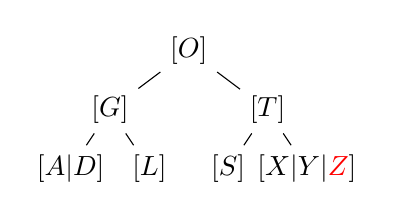
\begin{tikzpicture}[scale=0.5,
  level 1/.style={sibling distance=40mm},
  level 2/.style={sibling distance=20mm},
  level 3/.style={sibling distance=20mm},
  level 4/.style={sibling distance=20mm}]
\node{$[O]$}
	child{node{$[G]$}
		child{node{$[A|D]$}}
		child{node{$[L]$}}}
	child{node{$[T]$}
	child{node{$[S]$}}
	child{node{$[X|Y|\textcolor{red}{Z}]$}}};
\end{tikzpicture}\\

$\Rightarrow$ Der Knoten $[X|Y|\textcolor{red}{Z}]$ hat zu viele Einträge $\rightarrow$ Balancieren

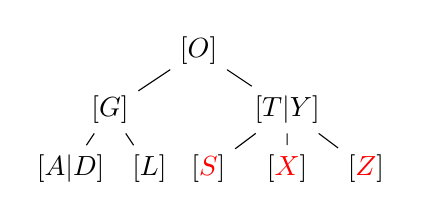
\begin{tikzpicture}[scale=0.5,
  level 1/.style={sibling distance=45mm},
  level 2/.style={sibling distance=20mm},
  level 3/.style={sibling distance=20mm},
  level 4/.style={sibling distance=20mm}]
\node{$[O]$}
	child{node{$[G]$}
		child{node{$[A|D]$}}
		child{node{$[L]$}}}
	child{node{$[T|Y]$}
		child{node{$[\textcolor{red}{S}]$}}
		child{node{$[\textcolor{red}{X}]$}}
		child{node{$[\textcolor{red}{Z}]$}}};
\end{tikzpicture}\\

$\Rightarrow$ Der Knoten $[T|Y]$ hat zu viele Kinder $\rightarrow$ Balancieren

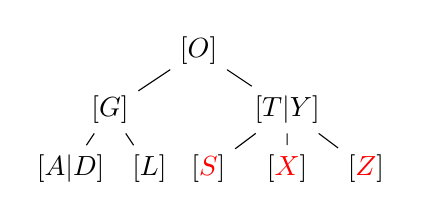
\begin{tikzpicture}[scale=0.5,
  level 1/.style={sibling distance=45mm},
  level 2/.style={sibling distance=20mm},
  level 3/.style={sibling distance=20mm},
  level 4/.style={sibling distance=20mm}]
\node{$[O]$}
	child{node{$[G]$}
		child{node{$[A|D]$}}
		child{node{$[L]$}}}
	child{node{$[T|Y]$}
		child{node{$[\textcolor{red}{S}]$}}
		child{node{$[\textcolor{red}{X}]$}}
		child{node{$[\textcolor{red}{Z}]$}}};
\end{tikzpicture}\\

\item remove(Z):
\item remove(A):
\item remove(L):


\end{enumerate}
\end{multicols}
\newpage
\noindent
\textbf{b)} Wiederholen Sie die Teilaufgabe (a) mit einem (2, 4)-Baum. \\




\begin{verbatim}
min children: 2, max children: 4
min entries: 1, max entries: 3
A,B,C,D,E,F,G,H,I,J,K,L,M,N,O,P,Q,R,S,T,U,V,W,X,Y,Z

insert(A):
              -----
              | A |
              -----
insert(L):
              ---------
              | A | L |
              ---------
insert(G):
              -------------
              | A | G | L |
              -------------
insert(O): first split
                 -----
                 | G |
                 -----
               /       \
              /         \
           | A |        | L | O |
insert(D):
                 -----
                 | G |
                 -----
               /       \
              /         \
         | A | D |     | L | O |
insert(T): second split
                 ---------
                 | G | O |
                 ---------
               /     |    \
              /      |     \
         | A | D | | L |   | T |
insert(S): 
                 ---------
                 | G | O |
                 ---------
               /     |    \
              /      |     \
         | A | D | | L |   | S | T |
insert(X):
                 ---------
                 | G | O |
                 ---------
               /     |    \
              /      |     \
         | A | D | | L |   | S | T | X |
insert(Y): rebasing the root -> third split
                 ---------------
                 | G    |    T |
                 ---------------
                /       |        \
               /        |         \
         | A | D | | L | O | S | | X | Y |
insert(Z):
                 ---------------
                 | G    |    T |
                 ---------------
                /       |        \
               /        |         \
         | A | D | | L | O | S | | X | Y | Z |
```
Starting tree:
                 ---------------
                 | G    |    T |
                 ---------------
                /       |        \
               /        |         \
         | A | D | | L | O | S | | X | Y | Z |

delete(Z): delete from leaf
                 ---------------
                 | G    |    T |
                 ---------------
                /       |        \
               /        |         \
         | A | D | | L | O | S | | X | Y |

delete(A): delete from leaf -> min 1 key required -> condition holds true
                 ---------------
                 | G    |    T |
                 ---------------
                /       |        \
               /        |         \
         | D |     | L | O | S | | X | Y |

delete(L): delete from Leaf -> 2 keys pressed -> node requirements 
satisfied -> G < O and S < T -> Order condition satisfied.

                 ---------------
                 | G    |    T |
                 ---------------
                /       |        \
               /        |         \
         | D |     | O | S |   | X | Y |


\end{verbatim}



